\section{Exact failures and a uniform wrong-sign regime}\label{sec:failures}
\subsection{Collision, early covered error and prefix dependence}
The nonlinear map does not automatically eliminate the exact two-pair obstruction. Under the original quarter-lag round-and-clip rule, the histories $[-,+]$ and $[+,-]$ still collide at all three widths. To see this, after one positive pair the blocks are $(p,-p)$ and $(-d_0,d_0)$. The opposite pair sends both to $(p-d_0,-p+d_0)=(2a,-2a)$; the required intermediate values are inside their relevant caps for the listed widths. The reversed history exchanges equal blocks. At width 12 the full code state is
\begin{equation}\label{eq:clipcollision}
 (k_\mu,r_+,i_+,r_-,i_-)=(2047,334,-334,334,-334).
\end{equation}
Both abstain, their completion metadata agrees, and their final labels differ.

The earliest lexical \emph{covered} error in the retained binary-label tree is $[-,-,+]$, at starts $0,4,8$. Two negative pairs leave blocks $(-52,52)$ and $(720,-720)$ at width 12. Applying the final positive map gives
\begin{equation}\label{eq:three}
 (2047,308,-308,694,-694),\qquad
 \etaosc=\frac{308^2-694^2}{308^2+694^2}
       =-0.6708967909800521\ldots .
\end{equation}
Its last label is positive. The wrong negative answer is outside the band. Length one is correct, and the only opposite-label length-two histories are the collision; equal-label histories remain correct. Thus length three is the first possible covered error in this declared tree. The harmonic state here has not reached either corner.

Eight identical final labels also need not erase a prefix. Consider zero-start negative prefixes of lengths $n=32$ and $n=128$, followed by eight positive pairs. The negative prefix leaves the minus block at $C_*$ and the plus block at
\[
 \Bmap^n(0,0)=\bigl(\max(\lambda,-nd_0),\min(\upsilon-a,nd_0)\bigr).
\]
At width 12, the two terminal plus blocks are respectively $(2047,-2048)$ and $(832,-1000)$; the terminal minus block in both is $D_8=(1672,-1840)$. Hence
\begin{equation}\label{eq:eightsuffix}
 \eta_{32,+^8}=0.15126835330983474\ldots,\qquad
 \eta_{128,+^8}=-0.5701419258344036\ldots .
\end{equation}
These are exact integer-state calculations followed by a rational norm ratio. They have the same last eight labels and opposite predictions. They do not share identical absolute completion metadata, so this example establishes prefix dependence of the fixed harmonic readout, not the stronger equal-metadata collision claim of \eqref{eq:clipcollision}. Adding integer start shifts could align clocks without changing baseline phases, but no additional trial is needed for the stated prefix-dependence result.

The retained constant-prefix reversal controls test both initial signs, both bases, all three widths, prefix lengths 32/128 and opposite suffix lengths $1,2,4,8,16,32$. One-pair reversals fail in directional coordinates at every width. Suffix lengths 16 and 32 succeed for the directional controls, consistent with the sufficient twelve-pair entrance proof. Alternating-prefix controls are retained separately. No success at these lengths is promoted to a minimal overwrite bound.

\subsection{What a finite tree says about information}
The saved exhaustive tree contains all $2^1+\cdots+2^{12}=8190$ zero-start histories per width and basis, 49,140 endpoints in total. It is not the full four-coordinate code grid or all lengths. At depth 12, each directional width has 54 distinct states, with 2,972 correct and 1,124 covered wrong decisions among 4,096 histories, and no abstentions. There are no opposite-last-label collision states at that particular depth.

The Fourier tree at depth 12 has 13 states, 2,048 correct, 924 abstentions and 1,124 covered wrong decisions; 11 states have opposite last labels. Earlier directional collisions coexist with later finite label separation. The absence of a collision at one depth does not make the frozen norm-sign decoder correct there, nor establish arbitrary-length capacity. Conversely, a wrong decoder output is not by itself proof that the state contains no label information. No new decoder is fitted to the finite tree.

\subsection{One-eighth lag: exact endpoint and all-grid proof}
Change only the lag to $1/8$, keep amplitude one, aligned starts $4m$, width 12, $H=2$, the original asymmetric interval, fixed global origin and event-wise rounding/clipping. This lag is inside the isolated-pair timing domain. The failure below is not a half-period alias.

Let $c_0,s_0$ be as in \eqref{eq:cs}, and define
\[
 e=\frac{s_0-c_0}{\sqrt2}>0,\qquad
 f=\frac{s_0+c_0}{\sqrt2},\qquad
 e_0=\rint(e/\Delta)=18,\quad f_0=\rint(f/\Delta)=255.
\]
Their strict rounding cells are rationally certified. The equality $f_0=w=255$ is only an equality of rounded codes; $f$ and $B_1/4$ are not identical.

\begin{theorem}[All-grid finite-entry reversal]\label{thm:eighth}
Under precisely these ideal-map assumptions, from any incoming harmonic grid state and any incoming mean, every label sequence of length at least 67 has a final fixed-readout sign opposite to its final label. The two terminal harmonic signatures, in code units, are
\begin{equation}\label{eq:signature}
 \ell=+1:\quad(\upsilon,\lambda+e_0,\upsilon-e_0,\lambda),
 \qquad
 \ell=-1:\quad(\upsilon-e_0,\lambda,\upsilon,\lambda+e_0).
\end{equation}
For both,
\begin{equation}\label{eq:wrongmargin}
 \ell N_{\rm dir}=2e_0(\upsilon+\lambda)\Delta^2
       =-\frac9{262144},\qquad
 \ell\etaosc=-2.16577126062446\,10^{-6}\ldots .
\end{equation}
The bound 67 is sufficient, not claimed minimal.
\end{theorem}
\begin{proof}
For LQ the early event is the first row of \eqref{eq:events}. At phase $\pi/4$, the late L event has harmonic increment $(f,e,-e,-f)$. UQ's late U event has $(-e,-f,f,e)$, exchanging the eventual block roles. Non-half-cell translation therefore gives the following LQ block actions:
\begin{equation}\label{eq:eighthmaps}
 \begin{aligned}
 r_+'&=\min(\upsilon,r_++a+f_0),&
 i_+'&=\max(\lambda+e_0,i_+-(b_0-e_0)),\\
 r_-'&=\min(\upsilon-e_0,r_-+a-e_0),&
 i_-'&=\max(\lambda,\min(\upsilon-f_0,i_--(f_0-b_0))).
 \end{aligned}
\end{equation}
For example, the plus imaginary composition first subtracts $b_0$, clips below, then adds $e_0$; the upper clip is redundant because $b_0>e_0$. The minus real composition first adds $a$, then subtracts $e_0$; its lower clip is redundant because $a>e_0$. UQ exchanges these two block maps. Thus, under either label, each real code satisfies
\begin{equation}\label{eq:drift}
 r'\ge\min(\upsilon-e_0,r+149),\qquad
 i'\le\max(\lambda+e_0,i-62)
\end{equation}
for each imaginary code. Indeed $a-e_0=149$, $a+f_0=422\ge149$; $b_0-e_0=175\ge62=f_0-b_0$. The extra upper cap in the last line of \eqref{eq:eighthmaps} can only decrease its output, preserving the upper comparison.

Monotonicity allows iteration of these scalar comparisons for any sequence of labels. Starting with $r\ge\lambda$ gives
$r_n\ge\min(\upsilon-e_0,\lambda+149n)$.
Starting with $i\le\upsilon$ gives
$i_n\le\max(\lambda+e_0,\upsilon-62n)$.
The distance to the required boundaries is $2K-1-e_0=4077$; hence
\[
 n_r=\lceil4077/149\rceil=28,\qquad
 n_i=\lceil4077/62\rceil=66 .
\]
All four harmonic coordinates lie in
\begin{equation}\label{eq:rectangle}
 \mathcal R=\bigl([\upsilon-e_0,\upsilon]\times
                         [\lambda,\lambda+e_0]\bigr)^2
\end{equation}
after at most 66 pairs. The comparisons show that these lower/upper thresholds persist; the global code caps give the other two sides, so $\mathcal R$ is invariant.

Now take an incoming state in $\mathcal R$ and apply LQ. The plus real coordinate reaches $\upsilon$ since $a+f_0\ge e_0$; the minus real coordinate reaches $\upsilon-e_0$ since $a\ge e_0$. The plus imaginary coordinate reaches $\lambda+e_0$ since $b_0-e_0\ge e_0$. The minus imaginary coordinate reaches $\lambda$ since $f_0-b_0\ge e_0$. These are the literal inequalities $422\ge18$, $167\ge18$, $175\ge18$, $62\ge18$. Thus the next pair gives \eqref{eq:signature}; UQ exchanges the blocks. Both signatures lie in $\mathcal R$, so every subsequent pair again produces its own corresponding signature. This proves the arbitrary-label statement from pair 67 onward.

The label-signed squared-norm difference is
\[
 \upsilon^2+(\lambda+e_0)^2-(\upsilon-e_0)^2-\lambda^2
 =2e_0(\upsilon+\lambda)=-36 .
\]
Since $\Delta=1/1024$, this is $-9/262144$ in coefficient-squared units. The positive denominator is
\[
 [2047^2+(-2030)^2+2029^2+(-2048)^2]/1024^2
 =15.8522167205810546875 .
\]
Division gives \eqref{eq:wrongmargin}. Its magnitude is greater than $64\epsilon_{64}$, so the fixed rule resolves a strictly wrong sign rather than abstaining. The independent mean coordinate never enters this comparison.
\end{proof}
The retained 48 binary64 endpoints agree with these signatures. They are implementation instances, not a formal guarantee for every platform's arithmetic. The universal theorem rests on the ideal integer compositions and certified constants, not on the sampled histories or the earlier quarter-lag scalar-grid audit.

The two signatures are still label-dependent; the frozen energy-sign readout interprets them backwards. Reversing a sign for one known cell would be a new decoder design, not an information theorem or a universal repair. If one algebraically substitutes symmetric endpoints, the expression $2e_0(\upsilon+\lambda)$ becomes zero. That hypothetical combined eighth-lag/symmetric-endpoint control was not executed or adopted. No sign or endpoint is changed here.

\begin{figure}[ht]
\centering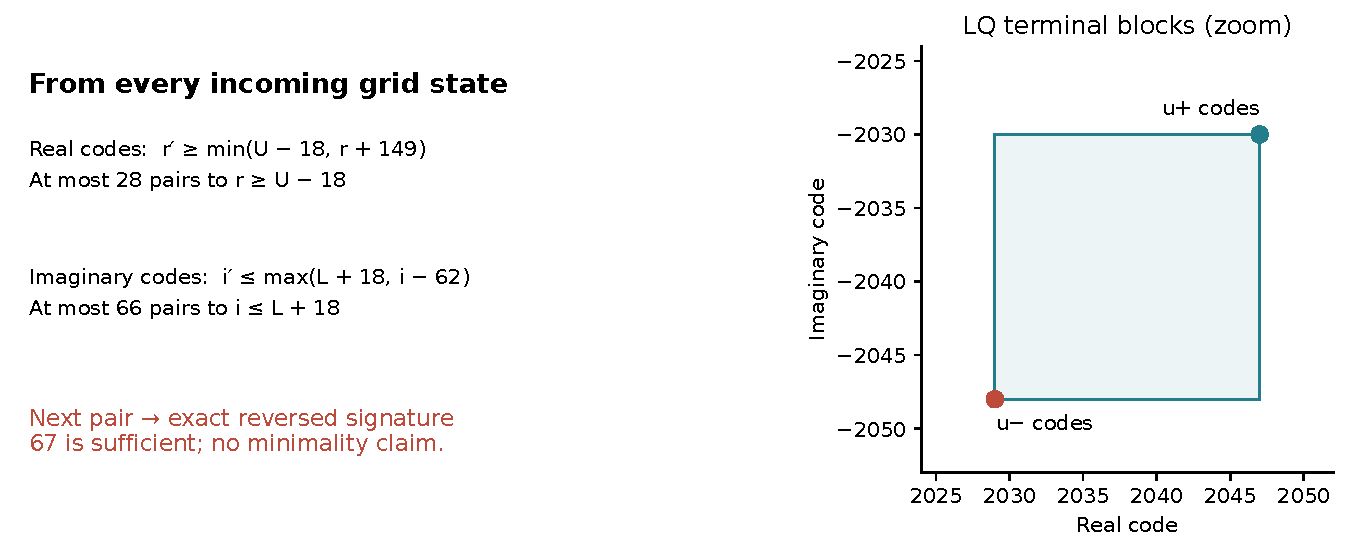
\includegraphics[width=\linewidth]{figures/fig05_eighth.pdf}
\caption{A sufficient all-grid proof, not a simulated convergence plot; $U=\upsilon$ and $L=\lambda$. Scalar comparisons put every block in the invariant rectangle by pair 66; the next pair creates the reversed signature. The zoom shows its two LQ blocks in numerical code space.}
\label{fig:eighth}
\end{figure}
